\documentclass[11pt,a4paper]{report}
\usepackage[utf8x]{inputenc}
\usepackage[T1]{fontenc}
\usepackage{fancyhdr} % only used to make the introduction page look nice
%\usepackage{gentium}
\usepackage{mathptmx} % Use Times Font
%
% Taken very gladly from Robert Jones
\usepackage[
    backend=biber,
    style = numeric
    ]{biblatex}

% Fill out the location of your references
\addbibresource{SNAIL.bib}

%%%
\usepackage{soul}
\usepackage{amsmath}
\usepackage{float}
\usepackage{ragged2e}
\usepackage{xcolor}
\usepackage{mathtools}
\DeclarePairedDelimiter\bra{\langle}{\rvert}
\DeclarePairedDelimiter\ket{\lvert}{\rangle}
\DeclarePairedDelimiterX\braket[2]{\langle}{\rangle}{#1\,\delimsize\vert\,\mathopen{}#2}
\DeclarePairedDelimiterX\braketmid[3]{\langle}{\rangle}{#1\,\delimsize\vert\,#2 \vert\,\mathopen{}#3}

\usepackage[%
  bookmarks=false,
  colorlinks,
  linkcolor=blue,
  urlcolor=blue,
  citecolor=blue,
  plainpages=false,
  pdfpagelabels,
  final,
  breaklinks=true
]{hyperref}

\usepackage{multicol}

\usepackage[pdftex]{graphicx} % Required for including pictures
%\usepackage{calc} % To reset the counter in the document after title page
%\usepackage{enumitem} % Includes lists

\frenchspacing % No double spacing between sentences
\linespread{1.05} % Set linespace
\usepackage[a4paper, 
lmargin=0.15\paperwidth, rmargin=0.15\paperwidth, tmargin=0.1\paperheight, bmargin=0.12\paperheight]{geometry} %margins
%\usepackage{parskip}

%\usepackage[all]{nowidow} % Tries to remove widows
\usepackage[protrusion=true,expansion=true]{microtype} 
\usepackage{titlesec} % This makes the chapter titles not have the annoying 'Chapter 1' header
\titleformat{\chapter}[display]
  {\normalfont\huge\bfseries}{}{0pt}{\Huge}

\date{}

\author{Alex Benitez}


\begin{document}

\begin{titlepage}
    \centering
    \vspace*{3cm} % Adjust vertical space at the top
    
    % Large Title
    {\LARGE\bfseries Calculating the Harmonic Response of Gas Particles Using the SFA Approximation \par}
    
    \vspace{0.5cm}
    
    % University Name
    {\Large King's College London \par}
    
    \vspace{0.5cm}
    
    % Course and Project Info
    {\large 6CCP3131 Third Year Project \par}
    
    \vspace{0.5cm}
    
    % Author's Name
    {\large \textbf{Alex Benitez} \par}
    
    \vspace{0.5cm}
    
    % Supervisor's Name
    {\large Supervisor: \textbf{Amelle Zaïr }\par}

    \vspace{2cm}
    {\small \textbf{Abstract:} Machine Learning for image recognition requires large datasets to be trained. High Harmonic Generation is a very computationally expensive process to simulate, inhibiting the ability to train Neural Networks without experimental data. This report outlines an Open-Source package called SNAIL, which greatly speeds up calculation of the HHG spectrum generated by various types of particles and customizable strong fields.}  %Modify before sending off
    
    
    \vfill % Push everything above to the center vertically
    \includegraphics[width=0.5\textwidth]{logosnail.png}
    
\end{titlepage}

% Bottom of the page
    %\includegraphics[width=4.19in]{SNAIL.jpg}\par\vspace{1cm}
\newpage
\tableofcontents
\newpage


\newgeometry{left=0.15\paperwidth, right=0.15\paperwidth, top=-0.065\paperheight, bottom=0.03\paperheight}

%\vspace{-20mm}
%\newgeometry{top=3cm, bottom=1.5cm, left=1.5cm, right=1.5cm}
\thispagestyle{fancy}
\setlength{\footskip}{0pt}
\chapter{Theoretical Background}
\vspace{-10mm}
\section{The Three Step Model}
Most nonlinear optical phenomena follow a simple relationship where the magnitude of the response drops linearly or exponentially with the order of the effect. In 1993 a series of experiments \cite{firstatto1}\cite{firstatto2} delivered a very surprising result, using high intensity lasers, a gas medium would generate a response with harmonics (pulses with multiples of the driving laser frequency) up to two orders of magnitude of the driving pulse, far exceeding any intuitive understanding. The simplest way to explain this result is with the three-step model, the origin of which is debated but generally attributed to \cite{threestep1}\cite{threestep2}\cite{threestep3}. In the model, a strong laser pulse deforms the potential well of an electron in an atom, the electron tunnels into the continuum at 0 velocity under the influence of the electric field, during a laser cycle it travels away and comes back to the atom, where it can scatter or recombine. Focusing only on the recombination, the electron will emit a pulse, equivalent to the kinetic energy gained in the continuum. This simple model allows for an intuitive understanding of most of the effects observed in High Harmonic Generation (HHG).
\\
\begin{figure}[h]

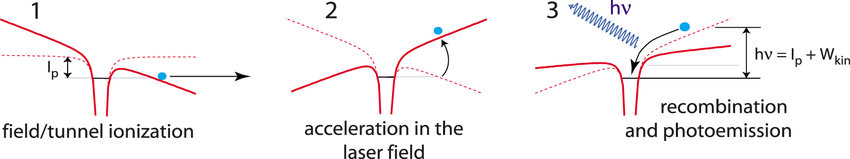
\includegraphics[width=1\textwidth]{threestep.jpg}
\caption{Graphic picturing the three step model of HHG, reprinted from \cite{Threestepfig}}
\end{figure}

Experimentally the maximum harmonic was found to be $I_p + 3U_p$ where $I_p$ is the ionization potential of the atom and $U_p = \frac{e^2 E^2}{4mw^{2}_o}$ is the ponderomotive energy, which is just the time averaged kinetic energy. Using the three step model, the maximum kinetic energy of the electron can be modelled, by considering a series of electrons under the influence of a simple laser the maximum kinetic energy is found to be around 3.17 $U_p$ which will have $I_p$ added to it as soon as the electron recombines, closely matching experimental results.

\begin{figure}[h]
\centering
\includegraphics[width=0.9\textwidth]{kineticplot.png}
\caption{Plot demonstrating the 1D trajectories of electrons released during positive electric field values. From top to bottom, the driving field, distance of the electron from the nucleus and the maximum kinetic energy at recombination. In the second plot the trajectory with the highest kinetic energy is black.}
\end{figure}
\newpage

\newgeometry{left=0.15\paperwidth, right=0.15\paperwidth, top=0.1\paperheight, bottom=0.12\paperheight}

\section{The Strong Field Approximation}
In 1994, Maciej Lewenstein and others introduced one of the most powerful tools to calculate HHG in a landmark paper \cite{lewensteinog}. The main assumptions of the Lewenstein model are: a) The ground state does not deplete, b) The ground state is the only bound state that affects the evolution of the system, c) The free electron only feels the external field, ignoring the atomic potential. For the ground state to not deplete, the ponderomotive force should be below $U_{sat}$, the saturation potential where all of the atoms ionize during interaction. Following the method set out in \cite{smirnovaMultielectronHighHarmonic2013}, \cite{propagators} and \cite{Emiliomasters}, for the remainder of the text except where explicitly stated we use atomic units. We start with the TDSE of one shell electron:

\begin{equation} 
	i\frac{\partial}{\partial t} \ket{\psi(t)} = \left[-\frac{1}{2} \nabla^2 + V(r) - Ecos(t)x\right] \ket{\psi(t)} = \hat{H}(t) \ket{\psi(t)}
	\label{TDSE}
\end{equation}
Here V(r) is the atomic potential, $Ecos(t)$ is the time-varying electric field from the driving pulse and $\hat{H}(t)$ is the Hamiltonian. What we want to find is the induced dipole, which is proportional to the response and given by:
\begin{equation}
\mathbf{D}(t) = \bra{\psi(t)}\hat{\mathbf{d}}\ket{\psi(t)}
\end{equation}
To calculate this, however, we need to represent the wavefunction in a convenient form; so we introduce propagators. A possible solution for \eqref{TDSE}, is:
\begin{equation}
\ket{\psi(t)} = e^{-i\int_{0}^{t} \hat{H}(t')dt'}\ket{\psi(0)} = e^{-i\int_{0}^{t} \hat{H}(t')dt'} \ket{g}
\end{equation}
Where we set the initial state of the wavefunction as $\ket{g}$ implying the electron starts in the ground state in the atomic well. However, this form is not actually useful; the Hamiltonian can be split into any two parts, which we choose as $\hat{H} = \hat{H}_0 + \hat{V}_L$. In this case $\hat{H}_0$ is the Hamiltonian of the atomic potential, and $\hat{V}_L$ is the interaction with the laser. To split it, we have to find an expression for the propagator of our full Hamiltonian, which we will call $U_1(t,t')$, first we assume:
\begin{equation}
i\frac{\partial}{\partial t}	U_0(t,t') = H_0 U_0(t,t') \qquad U_0(t,t) = 1
\end{equation}
and we want to solve:
\begin{equation}
i\frac{\partial}{\partial t}	U(t,t') = (H_0 + \Delta H)U(t,t') \qquad U(t,t) = 1
\end{equation}
The Dyson expansion states that this can be found recursively, and only taking the first term of the expansion since we neglect interaction with the atomic potential:
\begin{equation}
U(t,t') = U_0(t,t') \; -\; i\int^{t}_{t'} dt'' U(t,t'')\Delta H(t'') U_0(t'',t')
\end{equation}
A quick way to prove this is to substitute it in for itself which assumes knowledge of $U_0$ and U being a solution of itself and uses the Leibniz integral rule in the second line:
\begin{equation}
\begin{split}
i \frac{\partial U(t,t')}{\partial t} = i \frac{\partial}{\partial t} \left[-i \int^{t}_{t'} dt'' U(t,t'')\Delta H(t'') U_0(t'',t') + U_0)t,t')\right] \\
=U(t,t)\Delta H(t) U_0(t,t') + \int^{t}_{t'} dt'' i\frac{\partial U(t,t'')}{\partial t} \Delta H (t'') U_0(t'',t') + i\frac{\partial}{\partial t} U_0(t,t') \\
 = (H_0  + \Delta H) \int^{t}_{t'} dt'' U(t,t'')\Delta H (t'') U_0(t'',t') + \Delta H U_0(t,t') + H_0U_0(t,t') \\
= (H_0 + \Delta H )U(t,t')
\end{split}
\end{equation}

Finally, substituting in back for the exponential terms, the wavefunction can be expressed as:
\begin{equation}
\ket{\psi(t)} = e^{-i\int_{0}^{t} \hat{H}_0(t'')dt''}\ket{g} \; -\; i\int^{t}_{0}dt' \left[e^{-i\int_{t'}^{t} \hat{H}(t'')dt''}\right]\hat{V}_L(t')\left[e^{-i\int_{0}^{t'} \hat{H}_0(t'')dt''}\right]\ket{g}
	\label{propagatorfull}
\end{equation}
This very scary equation is surprisingly intuitive, the first standalone exponential term is the evolution of the non-ionized part of the electronic wavefunction. Inside the integral, the first exponential term acting on the ground state represents the evolution of the electron before it ionizes $\hat{H}_0(t'') = \hat{\mathbf{p}}^2/2 + U(\hat{\mathbf{r}})$; the $\hat{V}_L$ term indicates the transition from the ground state to the continuum, which happens at $t'$. The last term indicates the evolution and interaction with the electric field, which is why it includes the full Hamiltonian $\hat{H}$.


Equation \eqref{propagatorfull}, is still not very useful, since we still cant solve for the full Hamiltonian, here is where the assumptions of SFA shine. First, we assume that the Hamiltonian when the electron is in the laser field is given by $\hat{H_F} = \hat{H} - \hat{V}_A$, meaning we ignore the atomic potential. Luckily, the propagator for this case is known as the Volkov propagator, which when applied to an electron appearing in the continuum at $t'$ with momentum \textbf{p} and defining $\mathbf{A}(t) = -\int \mathbf{F}(t) \: dt$:
\begin{equation}
\begin{split}
\hat{U}_V(t,t')\ket{\mathbf{p} + \mathbf{A}(t')}\; & = \;e^{-iS_V(\mathbf{p},t,t')}\ket{\mathbf{p} + \mathbf{A}(t)} \\
S_V(\mathbf{p},t,t') \; &= \; \frac{1}{2}\int^{t}_{t'}dt''[\mathbf{p} + \mathbf{A}(t'')]^2 \\
\braket{\mathbf{r}}{\mathbf{p} + \mathbf{A}(t)} & = \frac{1}{(2\pi)^{3/2}} e^{i[\mathbf{p} + \mathbf{A}(t)]\cdot \mathbf{r}}
\end{split}
	\label{planewave}
\end{equation}
The physical explanation of this equation is, the electron enters the field from $t'$ to $t$ with momentum $\mathbf{p}$, by t, it has a momentum of $\mathbf{p} + \mathbf{A}(t)$ and a phase term of $e^{-iS_V(\mathbf{p},t,t')}$. From \eqref{planewave}, we know that the coordinate of the wavefunction is a plane wave, which at each moment in time forms a complete basis, meaning:
\begin{equation}
\int d\mathbf{p} \ket{\mathbf{p} + \mathbf{A}(t)} \bra{\mathbf{p} + \mathbf{A}(t)} = \hat{1}
	\label{identity}
\end{equation}

We can finally calculate the dipole over time, making the final assumptions that there is no permanent dipole in the ground state and the electron doesn't scatter or absorb extra energy from the field non-adiabatically:
\begin{equation}
\mathbf{D}(t) \: \approx \: -i\braketmid{\hat{U}_0 (t,t_0)g}{\hat{\mathbf{d}}}{\int^{t}_{t_0} dt' \hat{U_V}(t,t') \hat{V}_L(t') \hat{U}_0(t',t_0) \vert g} + c.c.
\end{equation}
Using identity \eqref{identity}, and expanding some terms, this takes the form of:
\begin{equation}
\begin{split}
\mathbf{D}(t) = i\int^{t}_{t_0} dt'' \int d\mathbf{p}\; \mathbf{d}^*(\mathbf{p} + \mathbf{A}(t))& e^{-iS(\mathbf{p},t,t')} \mathbf{F}(t') \mathbf{d} (\mathbf{p} + \mathbf{A}(t')) + c.c. \\
where \quad \mathbf{d}(\mathbf{p} + \mathbf{A}(t)) &= \braketmid{\mathbf{d}(\mathbf{p} + \mathbf{A}(t))}{\hat{\mathbf{d}}}{g}
\end{split}
	\label{analitical}
\end{equation}
Here the total action is used which includes the Ionization potential $I_p$. One last rearrangement gives us the form:
\begin{equation}
\begin{split}
\mathbf{D}(t) = i\int^{t}_{t_0}dt''\int \; d\mathbf{p} \: &\mathbf{d}^*  (\mathbf{p} + \mathbf{A}(t)) e^{-iS(\mathbf{p},t,t')} \Phi ( \mathbf{p} + \mathbf{A}(t'')) + c.c. \\
\Phi ( \mathbf{p} + \mathbf{A}(t'')) & = \left[\frac{(\mathbf{p} + \mathbf{A}(t''))^2}{2} + I_p\right]\braket{\mathbf{p} + \mathbf{A}(t'')}{g}
\end{split}
\end{equation} 

The final step to get the harmonic spectrum is to calculate the Fourier transform:
\begin{equation}
I(N\omega) \propto (N\omega)^4 \vert D(N\omega) \vert ^2
\end{equation}
\newpage
\section{The Saddle Point Method}
The previous section provided us with a very useful approximation, but if we were to try to calculate this, we would soon run into large rounding errors since the action term makes the integral highly oscillatory. The action oscillates much quicker than the rest of the terms in the integral, this means that the biggest contributions to the integral \eqref{analitical} are when the action varies slowly, since the response of the rest of the trajectories will destructively interfere. Additionally, due to our assumptions, the action is the difference in position of the electron between two different times, which leads to stationary points:
\begin{equation}
\nabla S(\mathbf{p},t,t') = \mathbf{x}(t) - \mathbf{x}(t')  = 0
\end{equation}
This tells us that the most 'relevant' trajectories are the ones that begina and end in the same place, which are the electrons that recombine. The action integral can be expanded:
\begin{equation}
\begin{split}
S(\mathbf{p},t,t') = \; & \int^{t}_{t_0} dt'' \left(\frac{(\mathbf{p} - \mathbf{A}(t''))^2}{2} + I_p \right) \\
=\; &\frac{1}{2} \mathbf{p}^2 (t - t') - \mathbf{p} \cdot \int^{t}_{t_0} \mathbf{A}(t'')dt'' + \int^{t}_{t_0} dt'' \left(\frac{\mathbf{A}(t'')^2}{2} + I_p \right)
\end{split}
\end{equation}
Here, the second term is 0, the integral of a potential over a closed loop is always 0, and our electron ends where it starts. The third term can be taken out of the momentum integral since it only depends on the field. Finally we can also assume the momentum integration will mostly be affected by the action integral and the dipole elements can be taken out:
\begin{equation}
i\int^t_{t_0} dt''\: \mathbf{d}^*  (\mathbf{p} + \mathbf{A}(t)) \mathbf{d}(\mathbf{p} + \mathbf{A}(t'))\mathbf{F}(t') e^{-i \int^t_{t_0} dt'' \left(\frac{\mathbf{A}(t'')^2}{2} + I_p \right)} \int d\mathbf{p} e^{-\frac{1}{2}i \mathbf{p}^2 (t - t')} + c.c.
\end{equation}
The last integral is very similar to a gaussian integral, and if we convert from integrating over return time, to integrating over total excursion time $\tau = t - t'$, and add a small factor$\epsilon$ to the exponent making it $exp(-i\frac{1}{2}p^2 (\tau - i \epsilon))$ it becomes a full gaussian, without losing much accuracy if the $\epsilon$ is small. The saddle point approximation states that we can take integrals of this form as:
\begin{equation}
\int F(\beta) e^{\rho\phi(\beta)} d\beta = \sum_s \sqrt{\frac{2\pi}{\rho}} \frac{F(\beta)e^{\rho\phi(\beta)}}{\sqrt{-\phi '' (\beta_s)}}
\end{equation}
Where the summation is over the saddle points, taking our saddle points that start and end in hte same place, we can finally write our integral in the form:
\begin{equation}
\mathbf{D}(t) = -\int_0^{\infty} d\tau \left( \frac{\pi}{\epsilon + i\tau/2}\right)^{3/2}\mathbf{d}^* (\mathbf{p}(t,\tau) + \mathbf{A}(t))\mathbf{d} (\mathbf{p}(t,\tau) + \mathbf{A}(t')) \mathbf{F}(t') e^{-iS(t,\tau)} + c.c.
	\label{FullIntegral}
\end{equation}
Where the action no longer depends on momentum, and the integral oscillates much more slowly. Despite a large number of approximations, except in the low harmonics, where our assumptions are not valid, this theory describes HHG very accurately. This is where a large majority of the processing time is taken up for SFA calculations, so optimization is essential. In the next chapter we will explore how vectorizing this integral using numpy can greatly speed up calculations.
\newpage
\newgeometry{left=0.15\paperwidth, right=0.15\paperwidth, top=-0.01\paperheight, bottom=0.12\paperheight}
\chapter*{SNAIL: An SFA library}
\vspace{-10mm}
The aim of this project was to develop an open-source python library which can numerically integrate \eqref{FullIntegral}. I aimed to make it as computationally efficient as possible, to allow for Machine Learning (ML) applications and landscape studies, where several factors in a simulation are slowly changed to reveal novel effects.
\section{Vectorization using Numpy}







%\begin{equation}
%\Psi^V_\mathbf{p} (\mathbf{r},t,t') \; = \; \frac{1}{(2\pi)^{3/2}}e^{-iS_V(\mathbf{p},t,t')}  %e^{i[\mathbf{p} + \mathbf{A}(t)]\cdot \mathbf{r}}
%\end{equation}

\printbibliography


\end{document}